\section{SEAS problems}
\subsection{Modeling Environment}
The applications are motivated by the study of quasi-static deformation of the solid Earth over the time scales of earthquake cycles.
In both the interseismic and coseismic phases, the off-fault material response is modeled as elastic-plastic.
\begin{equation}\label{eqn:governing}
    \rho \ddot{u} = \nabla \cdot \sigma + F, \sigma = \boldsymbol{C} : (\epsilon - \epsilon^p) 
\end{equation}

Here, $\rho$ is the material density, $u$ is the vector of particle displacements, $F$ is the body fordce, $\boldsymbol{C}$ is the stiffness tensor of elastic moduli, and $\epsilon$ and $\epsilon^p$ are the elastic and plastic strains.
\begin{figure}
    \centering
    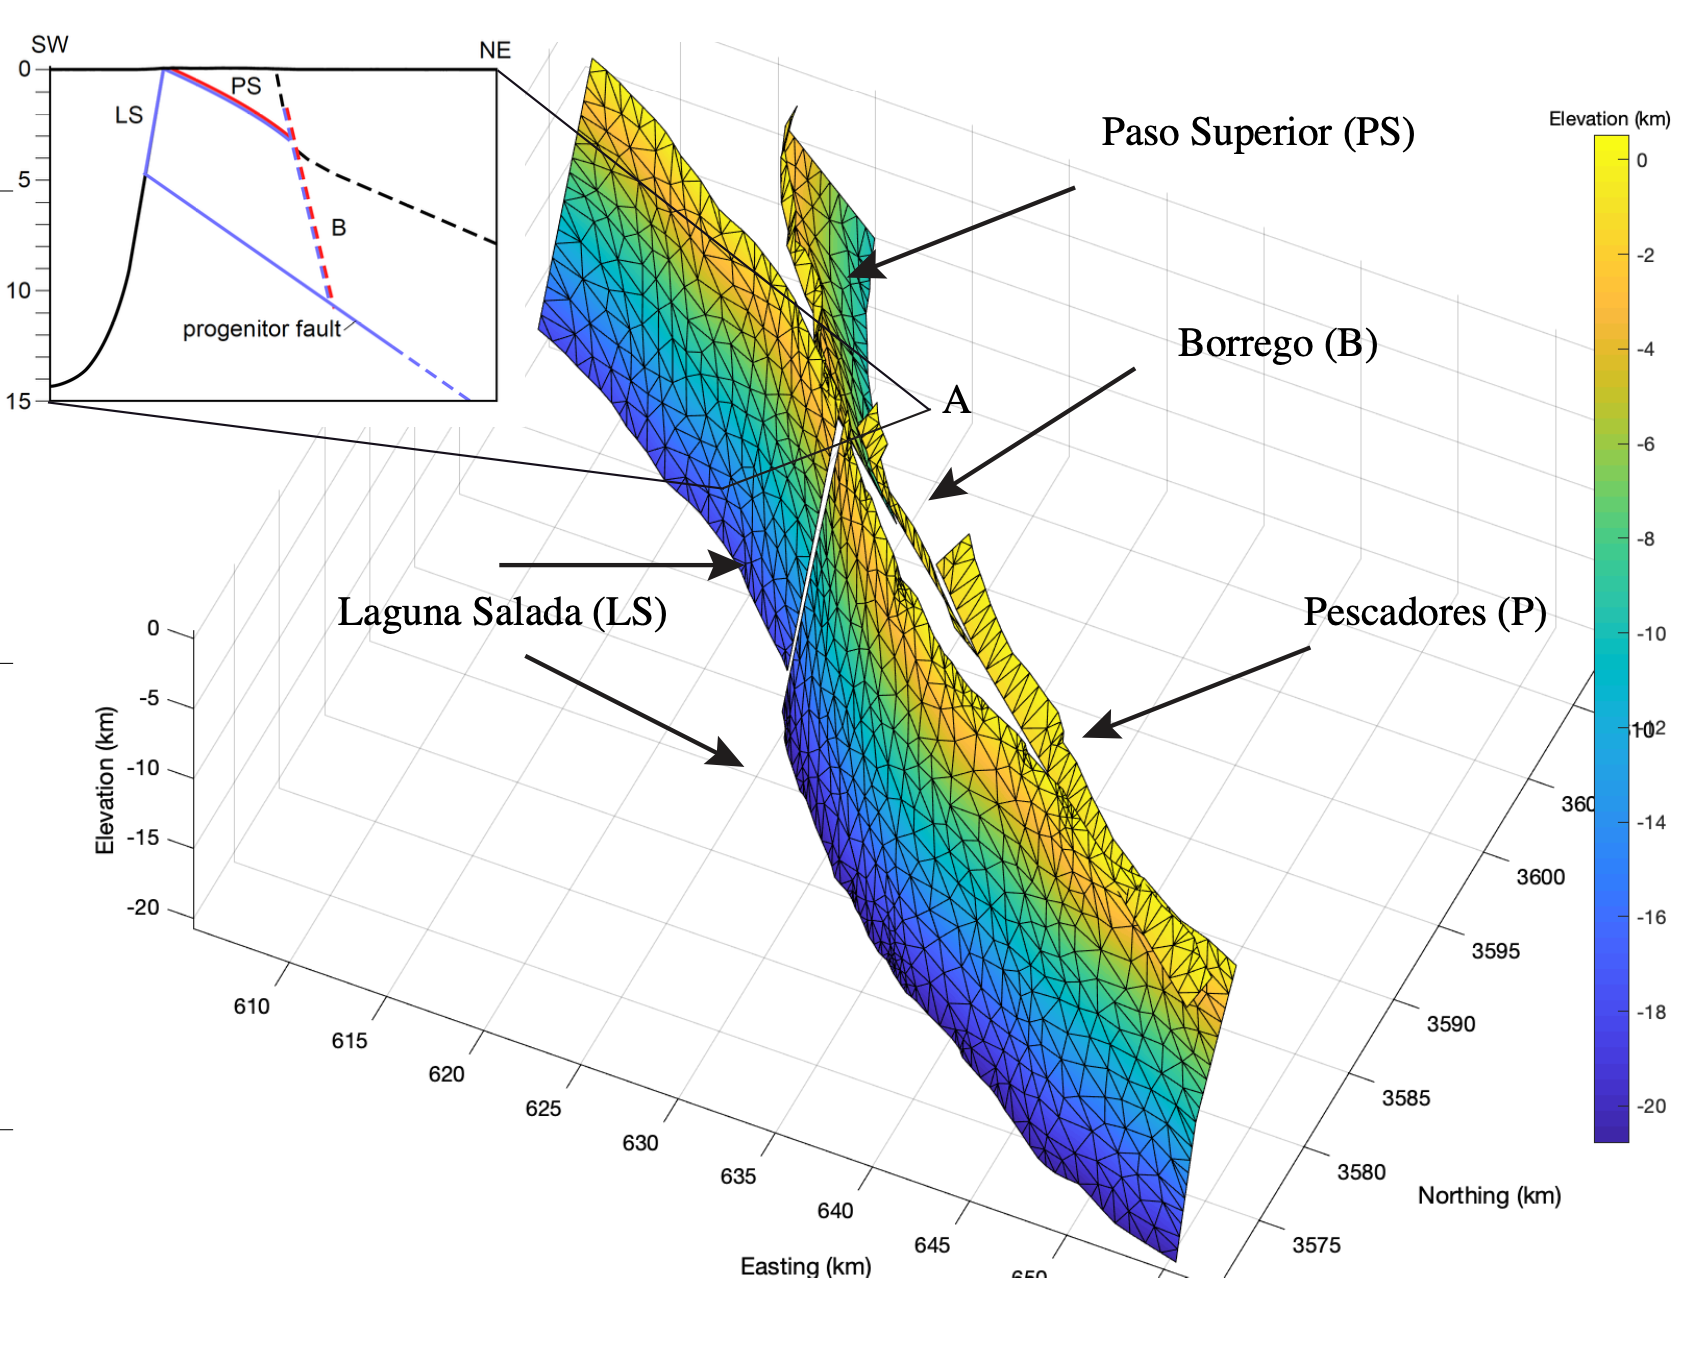
\includegraphics[width=\linewidth]{figures/fault-network.png}
    \caption{A 3D image of the complex fault network from EMC earthquake; image generated using scripts from \citep{https://doi.org/10.1002/2016GL072289}}
    \label{fig:fault-network}
\end{figure}
A fault network (an example shown in \autoref{fig:fault-network}) is composed of faults governed by non-linear, rate-and-state friction which determines the relationship between the slip velocity $V$ to shear traction $\tau$ with the (effective) norm stress $\bar{\sigma}$, the friction coefficient $f$ and a state variable $\Psi$.
\begin{equation}\label{eqn:friction-law}
    \tau = \bar{\sigma} f(V,\Psi), \Psi = G(V, \Psi)
\end{equation}
The form of the state evolution law $G$ can take several forms such as the aging law in which the state evolves in the absence of slip or the slip law with strong rate-weakening.

During the interseismic phase, the inertial terms in the governing \autoref{eqn:governing} are set 0 ($\ddot{u} = 0$).
Tectonic loading is imposed through time-dependent boundary conditions and the slip on faults are incorporated through friction law \autoref{eqn:friction-law}.
The evolution of $\Psi$ constraints the time step, and very large time steps can be used during the interseismic phase.
The main computational challenge comes from solving the large linear systems of equations that come from the discretization of the steady-state version of the \autoref{eqn:governing}.
During the interseismic phase, tectonic loading determines the boundary conditions and the stress on faults as the result of elastic deformation.
Once an event begins to nucleate, we enter the coseismic phase and inertial terms of governing \autoref{eqn:governing} are retained.
It is more efficient to use explicit integration during this period because it simplifies the computation. In both phases, the governing equation can be solved using the SBP-SAT methods mentioned in the previous section.

\subsection{3D Problem Setup}
The 3D problem setup described below is taken from previous SEAS publications \citep{10.1785/0220190248}.
The medium is assumed to be a homogeneous, isotropic, linear elastic half-space defined by
\begin{equation} \label{eqn:domain}
    \textbf{x} = (x_1, x_2, x_3) \in (-\infty, \infty) \times (\infty, \infty) \times (0, \infty)
\end{equation}
with a free surface at $x_3 = 0$ and $x_3$ as positive downward. A vertical, strike-slip fault is embedded at $x_1 = 0$, We use the notation ``+'' and ``-'' to refer to the different sides of the fault. 

We assume 3D motion, letting $u_i = u_i(\textbf{x}, t), i = 1, 2, 3$ denote the displacement in the $i$-direction.
Hooke’s law for linear elasticity is given by
\begin{equation}
    \sigma_{ij} = K\epsilon_{kk}\delta_{ij} + 2\mu (\epsilon_{ij} - \frac{1}{3} \epsilon_{kk}\delta_{ij})
\end{equation}
for bulk modulus $K$ and shear modulus $\mu$. The strain-displacement relations are given by 
\begin{equation}
    \epsilon_{ij} = \frac{1}{2} \left[\frac{\partial u_i}{\partial x_j} + \frac{\partial u_j}{\partial x_i}\right]
\end{equation}
The description of these benchmark problems can be found in \citep{erickson2018seas,jiang2020seas}.
To simulate the SEAS problems using the quasi-static method, it usually follows these steps.

\begin{algorithm}
    \caption{Quasi-static Formulation Algorithm}
    \begin{algorithmic}[1]
        \State \textbf{Step 1:} Initialize boundary conditions and state variables
        
        \While{simulation time not reached}
            \State \textbf{Step 2:} Solve steady-state problems to obtain displacements
            % \State \hspace{1em} In 2D, Solve Poisson's equation
            % \State \hspace{1em} In 3D Solve linear elasticity
            \State \hspace{1em} Linear solve of equations of static elasticity
            
            \State \textbf{Step 3:} Calculate stress from displacements
            
            \State \textbf{Step 4:} Calculate slip velocity using rate-and-state friction
            
            \State \textbf{Step 5:} Determine time step size ($dt$) using ODE solver
            
            \State \textbf{Step 6:} Integrate state variables using aging law and $dt$
            
            \State \textbf{Step 7:} Update boundary conditions using slip velocity and $dt$
        \EndWhile
    \end{algorithmic}
\end{algorithm}

The DifferentialEquations.jl package provides powerful adapted ODE solvers based on Runge-Kutta methods and useful ODE interfaces that allow us to modify data and write to outputs.
The key challenge here is step 2 which requires solving a large linear system that is formed with the SBP-SAT methods.
It's difficult to apply direct methods due to their high memory requirements and computational inefficiency. 
In the next two chapters, we will go into detail to first formulate the linear systems using the SBP-SAT methods and then apply HPC algorithms to solve such problems.


\subsection{Solving for rate-and-state friction}
Rate-and-state friction plays a central role in all SEAS problems. 
The friction coefficient function $f$ in SEAS problems is given as a regularized formulation
\begin{equation}
    f(V, \theta) = a \sinh^{-1} [\frac{V}{V_0} \exp{\frac{f_0 + b \ln(V_0 \theta / L)}{a}}]
    \label{eqn:friction-coefficient}
\end{equation}

$f_0$ represents the reference friction coefficient. $V_0$ represents slip rate, and $a$ and $b$ are rate-and-state parameters. For benchmark problem 1 and 5, $b$ is constant as $b_0$, but $a$ varies throughout computational domain \text{$\Omega$}{$_f$} in order to define velocity-weakening and velocity-strengthening regions. We will define them in respective sections differently.

The state variable $\theta$ evolves according to the aging law
\begin{equation}
    \frac{d\theta}{dt} = 1 - \frac{V\theta}{L}
    \label{eqn:aging-law}
\end{equation}

The fault strength is given as 
\begin{equation}
    \textbf{F} = \bar{\sigma}_n f(V,\theta) \frac{\textbf{V}}{V}
    \label{eqn:fault-strength}
\end{equation}
where \textbf{F} and \textbf{V} are vectors and $V$ is the norm of the \textbf{V}.
The rate-and-state friction where shear stress on fault is equal to fault strength \textbf{F}.
In Quadsi-static simulations, fault displacements are solved given governing equations and boundary conditions. 
Shear stress is calculated using displacements on fault.
In \autoref{eqn:fault-strength} and \autoref{eqn:friction-coefficient}, we can solve for $V$ and then calculate components of $V$ based on components of \textbf{F}. 
This significantly simplifies the calculation and improves numerical accuracy due to the magnitude differences between different components of \textbf{F} and \textbf{V}.

Once all parameters in \autoref{eqn:friction-coefficient} and \autoref{eqn:fault-strength} are known along shear stress calculated from displacements, it is common to apply Newton's method given in Algorithm \autoref{alg:newton} to solve the non-linear equation to obtain $V$.
\begin{algorithm}
\caption{Newton's Method}
\begin{algorithmic}[1]
\State Initialize $x_0$
\State Set tolerance $\epsilon$
\State Set maximum number of iterations $N_{\max}$
\For{$k = 0, 1, 2, \ldots, N_{\max}$}
    \State Compute $f(x_k)$ gradient $\nabla f(x_k)$
    % \State Compute Hessian $\nabla^2 f(x_k)$
    % \If{$\nabla^2 f(x_k)$ is not positive definite}
    %     \State Modify Hessian to be positive definite (e.g., $\nabla^2 f(x_k) + \lambda I$ where $\lambda > 0$)
    % \EndIf
    \State Determine search direction $d_k = -(\nabla f(x_k))^{-1}f(x_k)$
    \State Perform line search to find step size $\alpha_k$ such that $f(x_k + \alpha_k d_k) < f(x_k)$
    \State Update $x_{k+1} = x_k + \alpha_k d_k$
    \If{$\|\nabla f(x_{k+1})\| < \epsilon$}
        \State Convergence achieved
        \State \textbf{break}
    \EndIf
\EndFor
\Return $x_{k+1}$
\end{algorithmic}
\label{alg:newton}
\end{algorithm}

In our problem with high nonlinearity from the $\sinh^{-1}$ function, to improve numerical stability, we also need to apply the ``safe-guarded'' method.
One commonly used method is called bisection, it uses a similar approach to binary search. 
Based on the functional values of a close range $[x_L, x_r]$, it updates the search range of the root $x$.
Newton's method modified with Bisection is given in Algorithm \autoref{agl:newton-bisec}.

\begin{algorithm}
\caption{Newton's Method with Bisection}
\begin{algorithmic}[1]
\State Initialize $x_0$, bounds [$x_L$, $x_R$], and $x = (x_L + x_R) / 2$
\State Set tolerance $\epsilon_a$, $\epsilon_r$ and step size $\alpha_k = x_R - x_L$
\State Set maximum number of iterations $N_{\max}$
\For{$k = 0, 1, 2, \ldots, N_{\max}$}
    \State Compute $f(x_k)$ and gradient $\nabla f(x_k)$
    % \State Compute Hessian $\nabla^2 f(x_k)$
    \State Compute $f_L$, $f_R$ as $f(x_L), f(x_R)$  
    % \If{$\nabla^2 f(x_k)$ is not positive definite}
    %     \State Modify Hessian to be positive definite (e.g., $\nabla^2 f(x_k) + \lambda I$ where $\lambda > 0$)
    % \EndIf
    \State Determine search direction $d_k = -(\nabla f(x_k))^{-1} f(x_k)$
    \State Perform line search to find step size $\alpha_k$ such that $f(x_k + \alpha_k d_k) < f(x_k)$
    \State Update $x_{k+1} = x_k + \alpha_k d_k$
    \If{$x_k < x_L$ or $x_k > x_R$}
        \State $x_k = (x_L + x_R) / 2$
        \State $\alpha_k = (x_R - x_L) / 2$
    \EndIf
    \If{$f(x_k) * f_L > 0$  }
        \State $(f_L, x_L) = (f, x_k)$
    \Else
        \State $(f_R, x_R) = (f, x_k)$
    \EndIf
    
    
    \If{$\|\nabla f(x_{k+1})\| < \epsilon_a$ and $\|\alpha_k\| < \epsilon_a + \epsilon_r * (\|\alpha_k\| + \|x\|))$}
        \State Convergence achieved
        \State \textbf{break}
    \EndIf
\EndFor
\Return $x_{k+1}$
\end{algorithmic}
\label{agl:newton-bisec}
\end{algorithm}

Because $V$ is solved for each grid point independently, the above methods can be implemented using vectorized approach either on CPUs or GPUs.
Logical operations used in the control branch can be implemented using $masks$, which is a common technique in parallelization. 
The above calculations, although complex in numerical form and involving key concepts in earthquake cycle simulations and rate-and-state friction laws are actually very cheap and can be accelerated easily using vectorized operations. It is not the focus of this thesis.

\subsection{Methods of Lines}
Governing equations in SEAS problems, like many other PDEs, involve both time and space.
Methods of Lines (MOL) is a common approach to solving these PDEs.
The basic idea of MOL is to replace the spatial derivatives in PDE with algebraic approximations such as the SBP-SAT method in our work.
Once this is done, the spatial derivatives are no longer explicitly dependent on spatial independent variables.
Thus, the only variable left is $t$.
In other words, we have a system of ODEs that approximate the original PDE and use various ODE solvers to solve the original PDE.
Since ODE solver is not the focus of this thesis, we use the default and the mostly recommended ODE solver \texttt{tsit5()} provided in DifferentialEquations.jl \citep{TSITOURAS2011770}.
This is an adaptive ODE solver based on the Runge-Kutta pair of orders 5(4).
The numerical stability of ODE solvers plays an important role in numerical solutions to PDEs, and they affect the simulation results and running time significantly in our research. 
However, this thesis is on the spatial discretization part of the MOL using the SBP-SAT method, which we will discuss in the next section in detail for BP1 and BP5 separately.
Contents related to ODE solvers will only be briefly mentioned without detailed discussion and analysis.
